\documentclass{beamer}
\usepackage[utf8]{inputenc}

\usetheme{Madrid}
\usecolortheme{default}
\usepackage{amsmath,amssymb,amsfonts,amsthm}
\usepackage{txfonts}
\usepackage{tkz-euclide}
\usepackage{listings}
\usepackage{adjustbox}
\usepackage{array}
\usepackage{tabularx}
\usepackage{gvv}
\usepackage{lmodern}
\usepackage{circuitikz}
\usepackage{tikz}
\usepackage{graphicx}
\usepackage{caption}
\captionsetup{labelformat=empty}  % removes "Figure:"


\setbeamertemplate{page number in head/foot}[totalframenumber]

\usepackage{tcolorbox}
\tcbuselibrary{minted,breakable,xparse,skins}



\definecolor{bg}{gray}{0.95}
\DeclareTCBListing{mintedbox}{O{}m!O{}}{%
	breakable=true,
	listing engine=minted,
	listing only,
	minted language=#2,
	minted style=default,
	minted options={%
		linenos,
		gobble=0,
		breaklines=true,
		breakafter=,,
		fontsize=\small,
		numbersep=8pt,
		#1},
	boxsep=0pt,
	left skip=0pt,
	right skip=0pt,
	left=25pt,
	right=0pt,
	top=3pt,
	bottom=3pt,
	arc=5pt,
	leftrule=0pt,
	rightrule=0pt,
	bottomrule=2pt,
	toprule=2pt,
	colback=bg,
	colframe=orange!70,
	enhanced,
	overlay={%
		\begin{tcbclipinterior}
			\fill[orange!20!white] (frame.south west) rectangle ([xshift=20pt]frame.north west);
	\end{tcbclipinterior}},
	#3,
}
\lstset{
	language=C,
	basicstyle=\ttfamily\small,
	keywordstyle=\color{blue},
	stringstyle=\color{orange},
	commentstyle=\color{green!60!black},
	numbers=left,
	numberstyle=\tiny\color{gray},
	breaklines=true,
	showstringspaces=false,
}
\begin{document}

\title 
{2.8.32}
\date{september 19,2025}

\author 
{Navya Priya - EE25BTECH11045}
\graphicspath{./figs}

\frame{\titlepage}
\begin{frame}{Question}
 Ayush starts walking from his house to office. Instead of going to the office directly, he goes to a bankfirst, from there to his daughter school and then reaches the office what is the extra distance travelled by Ayush in reaching his office? If the house is situated at $(2,4)$,bank at $(5,8)$, school at $(13,14)$ and office at $(13,26)$ and coordinates are in km.
\end{frame}

\begin{frame}{Variables Taken}
\begin{table}[H]
\centering
\renewcommand{\arraystretch}{1}
\begin{tabular}{|m{1cm}|m{1cm}|}
\hline
  $\vec{H}$   &  $\myvec{2\\4}$ \\ \hline 
  $\vec{B}$   &  $\myvec{5\\8}$ \\ \hline
  $\vec{S}$   &  $\myvec{13\\14}$ \\ \hline
  $\vec{O}$   &  $\myvec{13\\26}$ \\ \hline
\end{tabular}
\end{table}
\end{frame}

\begin{frame}{Theoretical Solution}
Let us solve the given equation theoretically and then verify the solution computationally.\\

To calculate the extra ditsance travelled by Ayush, let d$_1$ be the distance from his home to office
\begin{align}
    \text{d}_1\,&=\,||\vec{O}-\vec{H}||\\[4pt]
    \,&=\,\sqrt{\myvec{\vec{O-H}}^\top\myvec{\vec{O-H}}}\\[4pt]
    \,&=\,\sqrt{605}\,\text{km}\brak{\approx 24.59}
\end{align}
\end{frame}

\begin{frame}{Theoretical Solution}
Let d$_2$ be the actual distance travelled by Ayush,
\begin{align}
    \text{d}_2\,&=\,||\vec{B}-\vec{H}||\,+\,||\vec{S}-\vec{B}||\,+\,||\vec{O}-\vec{S}||\\[4pt]
    \,&=\,\sqrt{\myvec{\vec{B-H}}^\top\myvec{\vec{B-H}}}\,+\,\sqrt{\myvec{\vec{S-B}}^\top\myvec{\vec{S-B}}}\,+\,\\&\sqrt{\myvec{\vec{O-S}}^\top\myvec{\vec{O-S}}}\\[5pt]
     \,&=\,27\text{km}
\end{align}

The extra distance travelled is,
\begin{align}
    \text{d}_2\,-\,\text{d}_1\,&=\,27-24.59\\[4pt]
    \,&=\,2.41\,\brak{\approx2.4\text{km}}
\end{align}
\end{frame}

\begin{frame}[fragile]{C code}
\begin{lstlisting}
#include <stdio.h>
#include <math.h>

// Function to calculate distance between two points
double distance(int x1, int y1, int x2, int y2) {
    return sqrt(pow(x2 - x1, 2) + pow(y2 - y1, 2));
}
\end{lstlisting}
\end{frame}

\begin{frame}[fragile]{Call C.py}
\begin{lstlisting}
import numpy as np
import numpy.linalg as LA
import matplotlib.pyplot as plt
import matplotlib.image as mpimg

# Load shared library
if platform.system() == "Windows":
    dist_lib = ctypes.CDLL("./distance.dll")
else:
    dist_lib = ctypes.CDLL("./distance.so")

# Function signature
dist_lib.extra_distance.argtypes = [ctypes.c_int, ctypes.c_int, ctypes.c_int, ctypes.c_int,
                                    ctypes.c_int, ctypes.c_int, ctypes.c_int, ctypes.c_int]
dist_lib.extra_distance.restype = ctypes.c_double
\end{lstlisting}
\end{frame}

\begin{frame}[fragile]{Call C.py}
\begin{lstlisting}

# Call the C function
extra = dist_lib.extra_distance(2, 4,   # house
                                5, 8,   # bank
                                13, 14, # school
                                13, 26) # office

print("Extra distance travelled:", extra, "km")

\end{lstlisting}
\end{frame}

\begin{frame}[fragile]{Plot.py}
\begin{lstlisting}
import numpy as np
import numpy.linalg as LA
import matplotlib.pyplot as plt
import matplotlib.image as mpimg

# Coordinates
H = (2, 4)
B = (5, 8)
S = (13, 14)
O = (13, 26)

# Path via B & S
x_via = [H[0], B[0], S[0], O[0]]
y_via = [H[1], B[1], S[1], O[1]]

# Direct Path
x_direct = [H[0], O[0]]
y_direct = [H[1], O[1]]

plt.figure(figsize=(6,6))
# Plot via B & S (blue path)
plt.plot(x_via, y_via, 'bo-', label="Via B & S")

\end{lstlisting}
\end{frame}

\begin{frame}[fragile]{Plot.py}
\begin{lstlisting}
# Plot direct path (green dashed)
plt.plot(x_direct, y_direct, 'g--', label="Direct Path")

# Label points
for point, name in zip([H, B, S, O], ['H', 'B', 'S', 'O']):
    plt.text(point[0]+0.3, point[1], f"{name} {point}", fontsize=10)

# Labels
plt.xlabel("X Coordinate (km)")
plt.ylabel("Y Coordinate (km)")
plt.title("Paths between H and O")
plt.legend()
plt.grid(True)

plt.show()
\end{lstlisting}
\end{frame}

\begin{frame}{Plot}
From the graph, theoretical solution matches with the computational solution.

\begin{figure}[H]
\centering
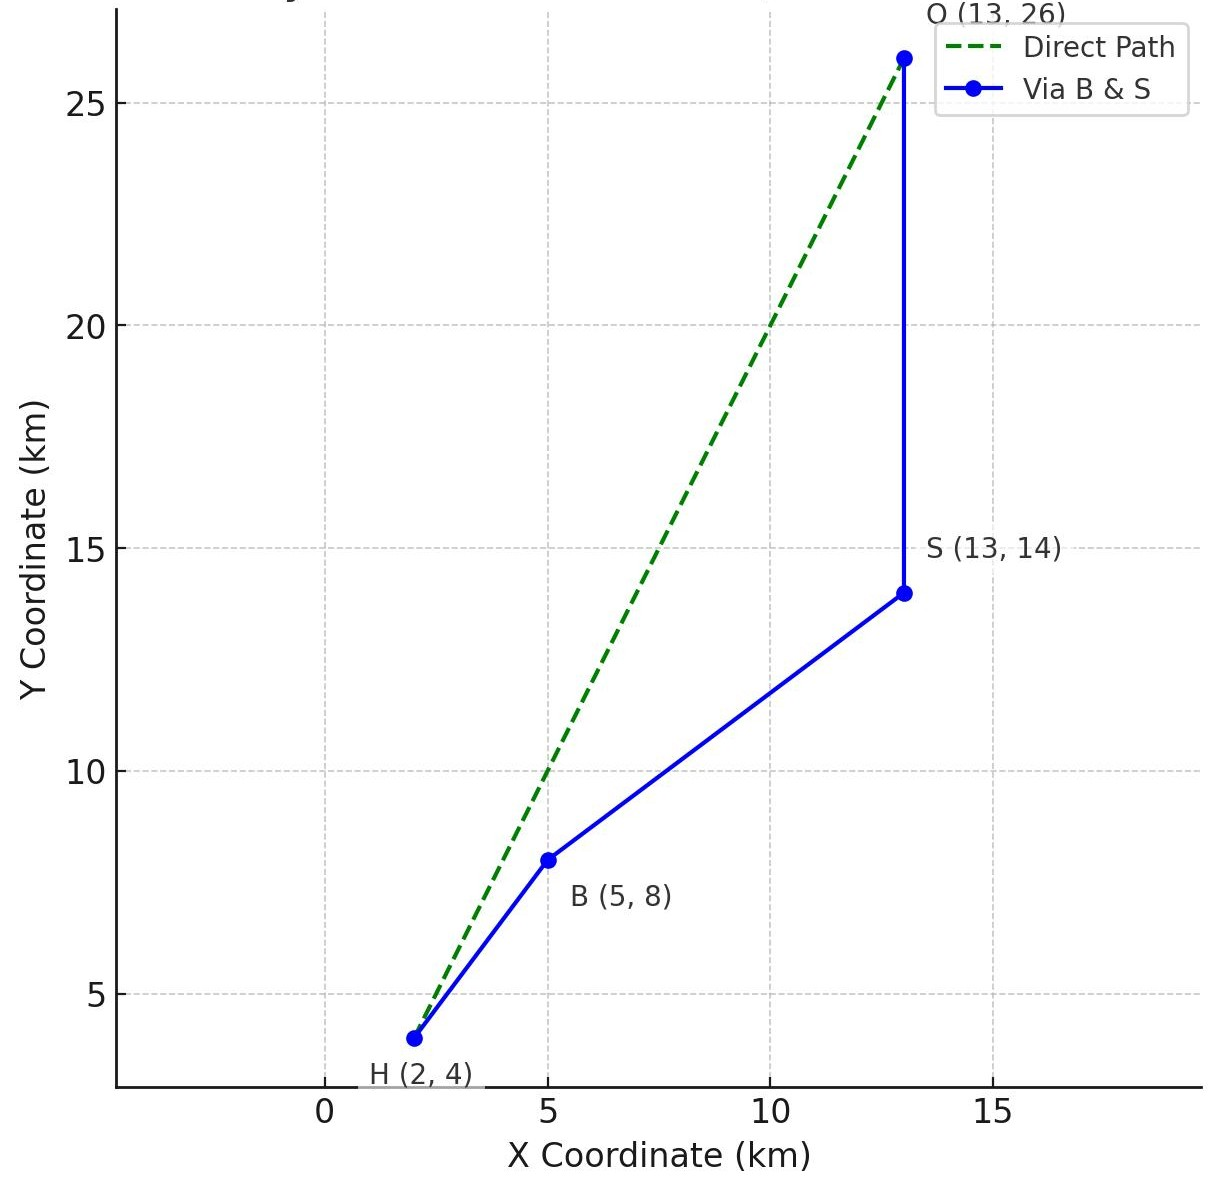
\includegraphics[width=0.5\columnwidth]{figs/graph.png}
 \caption*{Ayush's path to Office}
\label{fig:graph.png}
\end{figure}
\end{frame}
\end{document}